\documentclass[conference]{IEEEtran}

%%%%%%%%%%%%%%%%%%%%%%%%%%%%%%%%%%%%%%%%%%%%%%%%%%%%%%%%%%%%%%%%%%%%%%%%%%%%%%%%
%
% Package
%
%%%%%%%%%%%%%%%%%%%%%%%%%%%%%%%%%%%%%%%%%%%%%%%%%%%%%%%%%%%%%%%%%%%%%%%%%%%%%%%%
\usepackage{ifpdf}
\ifCLASSINFOpdf
  \usepackage[pdftex]{graphicx}
  % declare the path(s) where your graphic files are
  % \graphicspath{{../pdf/}{../jpeg/}}
  % and their extensions so you won't have to specify these with
  % every instance of \includegraphics
  \DeclareGraphicsExtensions{.pdf,.jpeg,.png}
\else
  % or other class option (dvipsone, dvipdf, if not using dvips). graphicx
  % will default to the driver specified in the system graphics.cfg if no
  % driver is specified.
  \usepackage[dvips]{graphicx}
  % declare the path(s) where your graphic files are
  % \graphicspath{{../eps/}}
  % and their extensions so you won't have to specify these with
  % every instance of \includegraphics
  \DeclareGraphicsExtensions{.eps}
\fi

\usepackage[utf8]{inputenc}
\usepackage[T1]{fontenc}
\usepackage[french, english]{babel}
\usepackage{cite}
\usepackage{caption}
\usepackage{amsmath,amsfonts,amssymb}
\usepackage{subcaption}
\usepackage{array}
\usepackage{float}
\usepackage{multicol}
\usepackage{algpseudocode}
\usepackage{algorithm}


\begin{document}
\pagestyle{plain}
\title{Submodular Optimization for Control of Prosumer Networks}


\author{Nicolas Gensollen, Vincent Gauthier, Monique Becker and Michel Marot  \\
\IEEEauthorblockA{CNRS UMR 5157 SAMOVAR, \\
Telecom SudParis/Institut Mines Telecom\\
Email: \{nicolas.gensollen, vincent.gauthier, monique.becker, michel.marot\}@telecom-sudparis.eu}}


\maketitle


\begin{abstract}
%The ability to control a given network by  dynamically injecting inputs offers ways to make sure that it stays in stable regions. In the case of smart grids, where end users exhibit complex behaviors and renewable production is quite unstable, control of the system  is paramount. 

In this paper, we study the case of a network composed of entities called prosumers. These agents have the ability to both consume and produce according to external conditions. We first design a model and simplify the underlying dynamic of such network using a second order coupled oscillators network model. Under some conditions, the system synchronizes to a common frequency. However, in case of perturbations in the power distribution, the system might lose synchrony and require control to bring it back to the stable state. In this situation, control can be seen as energy  absorbed or injected in the system at specific locations. Moreover, the power outputs of the prosumers are susceptible to change such that loads and generators are not fixed. In this context, it is important to select the right subset of nodes that yields, on average, the cheapest control in terms of energy. We propose and validate an algorithm based on a submodular optimization for chosing the driver nodes.
\end{abstract}


\IEEEpeerreviewmaketitle


\section{Introduction}
\label{sec:introduction}

Modernizing the power grid and increasing the share of renewables in the production are substantial objectives of the energetic transition. Because of progresses in communication, data management, and storage, the upcoming emergence of a power grid "2.0", often called smart grid, appears as a cross-disciplinary challenge of the 21st century \cite{Ramchurn}.

The today centralized top-down architecture is set to evolve to more distributed and bi-directional systems. Furthermore, the emergence of renewable and stochastic distributed energy resources (DER) in the distribution networks will require more flexibility. Within these systems, it is assumed that multiple aggregation levels will be required in order to organize and optimize communication. Agents responsible for generation and load portfolio managment, the so-called prosumers \cite{Parag2016} because they both produce and consume electricity, will provide services (generation, load shedding, frequency regulation) against remuneration \cite{Gensollen2014}. Insure grid stability within this uncertain context appears as a complex task. 

Several studies highlighted the need for increasing the storage capacity of the system. Some of them even consider electric vehicles as moving capacities that could be used for frequency regulation. In the case of fixed storage devices, the locations where they should be installed is an important question since it impacts the performances of the system. In a very static and top-down architecture, where loads and generators are fixed, this question is far from trivial. But in a smart grid scenario with bi-directional flows and agents that produce and consume depending on weather conditions, this becomes even more challenging. In this direction, \cite{Gkatzikis2015} studies the placement of storage equipments within microgrids in a collaborative scheme. The authors solve an interesting optimization problem mixing placement-dimensioning of storage with utilization. Moreover, \cite{Gkatzikis2015} uses a Nash bargaining framework to determine how prosumers should share the costs and benefits of the storages.


%More precisely, we are interested in the "best" locations for the storage equipments such that we are able to maintain stability when  perturbations occur. Since all nodes can switch from generator to load and vice versa, the optimal location is susceptible to change with the prosumers power output. Our goal is then to find the one that, on average, provides the best results.

%Since charging and discharging a battery is costly, we are particularly interested in the energy necessary to control the system when perturbations occur. The notion of performance of a given set of locations for using storage would then be inversely proportional to the energy used. One problem with this definition is that it depends explicitly on the state of the system and the prosumers power distribution. Besides, as the system size increases, the number of possible location sets increases exponentially. This forbid any algorithms using complete enumeration and evaluation of the sets. Moreover, we consider  that the electrical lines have maximum capacities, and storage equipments have both a maximum charge / discharge rate and  bounded capacities. Obviously, only solutions satisfying these constraints will be considered as feasible.

In this paper, we explore the use of storage in a network of prosumers whose power outputs are susceptible to change due to various external causes. In such a scenario with a high penetration of renewables, perturbations in the power distributions of the prosumers are very likely. Re-balancing the production and the consumption is then necessary and requires that we have the capability to control the grid's dynamic. Control of smart grid systems has been recently studied in \cite{Farraj2015}, where the authors use linear-quadratic optimal control theory in order to compute DER outputs. Control inputs rely on information collected by sensors and phasor measurement units and a communication network is used for sharing the information. The performances are then studied under practical limitations such as latency, sampling rate, or signal-to-noise ratio.

The present work differs in that we consider the control inputs as the actions of the storages on the grid dynamics. We are given a network of prosumers, and we have to find both the number and locations of the storages that should be deployed. Once this choice is made, we have to stick with it afterwards whatever the perturbations that may occur. We are thus looking for the smallest set of storages, as well as their locations, that will require a priori small control energy. Since we do not have any prior on the future perturbations, we minimize the average control energy required to move the system around the state space.

%If the balance between production and consumption is lost the system might desynchronize from the main frequency $\Omega$. If nothing is done to restaure synchrony, this could damage severely the generators and machines of the system. Since r


%, frequency regulation operators are paid to maintain synchrony in the meantime. Because charging and discharging storages is expensive (life cycles for instance), the less energy these operators use to control the frequency, the higher the profits. Furthermore, if we assume that we have a constrained budget, we are probably unable to place storage at every node in the network. That is, 

%We might expect that all sets of locations are not equal in term of the controllability that they provide. 


The power grid dynamic is represented by a coupled oscillator network. Each node, representing a prosumer, is modeled as an oscillator with a phase angle and a natural frequency that depends on its production/consumption. The oscillators are interconnected such that their frequencies are impacted by the ones of their neighbors. As we will see, the phase angles dynamics can be written as a system of coupled second order differential equations \cite{Filatrella2008}.

Optimal control theory can be used to compute the control inputs needed to restaure synchrony. However, there is no guarantee that these inputs will respect the physical constraints of the system. Electrical lines have indeed maximum capacities, and storages are also limited with bounded rates of charge/discharge which limit the possible inputs. We propose in this paper to incorporate these constraints in the model such that the control inputs remain realistic. Furthermore, we propose an optimization method that uses submodular set functions in order to find both the number of storages and their locations such that the average control energy required to maintain stability in this constrained system is minimized.


%Under some conditions, the system synchronizes and all nodes oscillates at $\Omega$. However, if a perturbation occurs, the system might desynchronize from $\Omega$ and requires control to bring it back to the stable synchronized state. Since the electrical lines and storages have finite capacities, we have further constraints on the control signals. Obviously, we do not wish to overload lines while trying to restaure synchrony. Likewise, no battery can inject power when empty, or charge/discharge quicker than some maximum rate. We propose in this paper to incorporate these constraints within the model such that the control signals remain realistic. 

This paper is organized as follows, section \ref{sec:control} presents recent advances about control in networks, section \ref{sec:The_Model} introduces the oscillator model designed for simplifying the grid's dynamic and derives the constraints on the control inputs. In section \ref{sec:control_and_submodularity} we propose an optimization method for finding the subset of driver nodes such that the average control energy is optimized. Finally, in section \ref{sec:Results}, we show some results and validation.



\section{Control in networks}
\label{sec:control}

In this section, we introduce some key notions related to the controllability of complex networks. We consider a graph $G=(V,E)$ of N nodes, where V is the vertex set and E is the edge set. The topology of this network can be encoded through the adjacency matrix M, which elements $m_{ij} \in \{0,1\}$ indicate whether i and j are connected. If the edges are weighted we can set $m_{ij} = w_{ij}$ where $w_{ij}$ is the weight of edge$(i,j)$, and zero if there is no edge. Graphs are often used to model complex interactions inside a population. Lets attribute to each node i the variable $ x_i $ that represents the state of node i. Depending on the model, this state can represent an opinion, a physical quantity, a probability and so on. If there is an edge between i and j, we might expect some interaction that would eventually change the values of $x_i$ and $x_j$. Such a dynamic is usually described with a system of differential equations. If we assume a linear first order dynamic, this can be written as $ \dot{X}(t) = A X(t) $, where $X(t)=\{x_0(t),...,x_{N-1}(t)\}$ is the vector of node states at time t, and matrix A encodes both the dynamics and the topology of the system (A can be, among other, the weighted adjacency matrix of the underlying graph).

If there is no action from the outside, the system state will evolve according to $ X(t) = X_0 e^{At} $ where $X_0$ is the initial state of the system. Imagine now, that this dynamic could be somehow influenced by injecting some signals. More precisely, lets assume that we can inject these signals in a subset of the nodes such that the dynamics becomes $ \dot{ X }(t) = A X(t) + B u(t) $, where the matrix B indicates which nodes receive the signals and $ u(t) $ is the vector of inputs at time t. Assume that the system is in some initial state $X_0$ and we aim at bringing it to some final state $X_T$ in some amount of time T. Control can be seen as finding the sequence of inputs $\{u(t_0),...u(t_T)\} $ that would do it given the dynamics A. Furthermore, we say that the system is controllable in T steps if it can be steered from any initial state $ X_0 $ to any final state $ X_T $ through a sequence of control inputs. 

It was shown by Kalman in 1963 that a linear system $(A,B)$ is controllable if the controllability matrix $ C = [B,AB,A^2B,...,A^{N-1}B] $ has full rank, that is, $rank(C) = N$. Nevertheless, when studying the controllability of non trivial networks, using the Kalman's criterion is not a simple task since matrix C becomes huge. Furthermore, because $A^k\longrightarrow 0$ when $k\longrightarrow \infty $, numeric precision becomes quickly an issue when computing the rank of C. A different approach to study controllability in complex network was introduced later on by Lin \cite{1100557}. This relates the search of the minimum driver set to a maximum matching in a bipartite graph, which can be done with the Hopcroft-Karp algorithm in $ O(|E|\sqrt{|V|}) $ in the worst case. This requires that the system $(A,B)$ is a structured system, meaning that all elements in A and B are either fixed zeros or independant free parameters. In such a situation, structural control is extremely powerfull since it enables us to discuss a network's controllability relatively quickly even if we do not know the exact weights of the edges. Note however that the independance of the parameters is a key assumption. If A is the adjacency matrix of an undirected network for instance, independance is not verified (since A is symetric). In this case, one should use different tools to study controllability \cite{Yuan2014}. 

The fact that a system is controllable or not is not the only criterion of interest. Indeed, if it is controllable, the amount of control energy required also appears as a key criterion. Actually, if the system is controllable, there might be more than one sequence of control inputs $u(t)$ that could drive it from $X_0$ to $X_T$. Among all these possibilities, optimal control is devoted to find the sequence that minimizes some cost function that can depend on the sates of the system $X(t)$, the control inputs $u(t)$, and the final state $X_T$. In the following, these control inputs will be used to model the actions of storage devices in a power grid. We are therefore particularly interested in the sequence that requires the minimum amount of control energy \cite{Yan2012}. Let $ \mathcal{E} = \int_{0}^{T} \Vert u(t) \Vert^2 dt $ be the energy used for the control of the system. It can be shown \cite{Liu2015} that the control inputs that minimize $ \mathcal{E} $ can be written as :


\begin{equation}
\label{eq:ustar}
 u^{\star}(t) = B^{T}e^{ A^{T}(T-t) } W^{-1}(T) v_f 
\end{equation}


where $ \nu_f = X_T - X_0 e^{AT} $ is the difference between the desired final state $X_T$ and the final free state $X_0 e^{AT} $, and $W(t) = \int_{0}^{t} e^{A \tau}BB^{T} e^{A^{T} \tau} d\tau $ is called the Gramian matrix of the system. It can also be shown that the system is controllable if and only if the Gramian is not singular, and that its rank indicates the dimension of the controllable subspace. Besides, the minimum control energy associated with the inputs $ u^{\star}(t)$ can be written as :


\begin{equation}
\label{eq:energy}
 \mathcal{E}_{min} = \nu_f^T W^{-1}(T) \nu_f
\end{equation}

In cases where W is not invertible, the pseudo-inverse $W^{\dagger}$ can be used to obtain similar information in the controllable subpsace. 

Until now, we stayed very general on the state variables and the dynamics of the system. In the following section, we use a coupled oscillators model as to encode the grid dynamics in some equation of the form $\dot{X}=AX$.



\section{Model design for power grid dynamics}
\label{sec:The_Model}

\subsection{Grid dynamic without constraint}

In this section, we introduce the coupled oscillators network model used to simplify the power grid dynamic. More details can be found in \cite{Filatrella2008}.

 The objective is to achieve synchronization of the grid at the main frequency $ \Omega = 50 Hz $. Each oscillator i has a phase angle $ \delta_i $ and a frequency $ \dot{\delta}_i $. Therefore, we seek an equilibrium of the form : $ \forall i,\ \dot{\delta}_i = \Omega $. For convenience, we express the dynamic of the oscillators in terms of the deviations from the main frequency : $ \delta_i(t) = \Omega t + \theta_i(t) $. Let $ \omega_i = \dot{\theta_i} $, such that $ \dot{\delta_i} = \Omega + \omega_i $. The equilibrium, in terms of the deviations dynamics, is : $ \forall i,\ \omega_i = 0 $

The next step consists in translating the dynamics of the generators and machines into equations involving the phase angles $ \theta_i $ and the frequencies $ \omega_i$. Generators and machines are composed of a turbine that dissipates energy at a rate proportional to the square of the angular velocity : 

\begin{equation}
\label{eq:diss}
  P_{diss, i}(t) = K_{Di}(\dot{\delta_i}(t))^2 
\end{equation}

where $ K_{Di} $ is the dissipation constant of entity i.

Furthermore, it also accumulates kinetic energy at a rate : 

\begin{equation} 
\label{eq:acc}
P_{acc,i}(t) = \frac{1}{2}I_i\frac{d}{dt} \left( \dot{ \delta_i }(t)^2 \right)
\end{equation} 

where $ I_{i}$ is the moment of inertia of entity i. For simplicity, we consider that all entities have the same dissipation constants($K_D$) and moment of inertia (I).

The condition for the power transmission between i and j is that the two devices do not operate in phase. The phase difference between i and j is : $ \delta_j(t) - \delta_i(t) = \Omega t + \theta_j(t) - \Omega t - \theta_i(t) = \theta_j(t) - \theta_i(t) $. The transmitted power along the line can be written as : 

\begin{equation}
\label{eq:trans}
 P_{transmitted} = - P_{ij}^{MAX} sin( \theta_j - \theta_i )
\end{equation}
  
with $ P_{ij}^{MAX} $ being the maximum capacity of the line $(i,j)$. Each entity i is then described by a power balance equation of the type :

\begin{equation}
\label{eq:bilan}
 P_{S,i}  =  P_{diss,i} + P_{acc,i} + P_{transmitted,i},
\end{equation}

where $ P_{S,i} $ is the power of an ideal source or sink at node i. By substituting equations \ref{eq:diss}, \ref{eq:acc}, and \ref{eq:trans} into equation \ref{eq:bilan} and re-arranging the terms, we obtain the following non-linear coupled system of equations :

\begin{equation}
\label{eq:without_simplification}
\begin{array}{lll}
P_{S, i}  =  I \Omega \ddot{ \theta_i }  + \left[ I \ddot{ \theta_i } + 2 K_D \Omega \right] \dot{ \theta_i } + K_D \Omega^2 \\+ K_D \dot{ \theta_i }^2 - \sum_{j \in \mathcal{N}_i} P_{ij}^{MAX} sin \left[ \theta_j - \theta_i \right] \end{array}
\end{equation}

We now use simplifications based on the fact that we consider small deviations from the main frequency : $ \dot{ \delta}_i \sim \Omega $ which means that $ \omega_i = \dot{\theta_i} << \Omega $, such that the squared term $ K_D \dot{\theta}_i^2 $ can be neglected.
Moreover, we assume that the rate at which energy is stored in the kinetic term is much less of the rate at which energy is dissipated by friction : $ \ddot{ \theta }_i  << \frac{2 K_D}{I} $ (see \cite{Filatrella2008} for more details). Equation \ref{eq:without_simplification} becomes :

\begin{equation}
 \ddot{ \theta_i } \sim \psi_i - \alpha \dot{ \theta_i } - \sum_{j\neq i} K_{ij} sin \left[ \theta_j - \theta_i \right],
\end{equation}

where $ \alpha = \frac{2 K_D}{I} $ is the dissipation term, $ K_{ij} = \frac{P_{ij}^{MAX}}{I \Omega} $ are the coupling strengths, $ \psi_i = \left[ \frac{P_{S,i}}{I \Omega} - \frac{K_D \Omega}{I} \right] $. In order not to overload the equations, we simplify the constant term $ \frac{K_D \Omega}{I} $ by working in a rotating frame such that $ \psi_i=\frac{P_{S,i}}{I \Omega} $.

The dynamic is still non linear because of the sine coupling. Therefore, we also assume that the phase angle differences are small such that $ sin \left[ \theta_j - \theta_i \right] \sim \theta_j - \theta_i $. By using vector notations, the dynamic can be written in the following form :

\begin{equation}
\label{eq:with_simplification}
\ddot{\theta} = \Psi - \alpha \dot{\theta} - (K \circ L)\theta
\end{equation}

Where $ A \circ B $ represents the Hadamard product between matrices A and B, and L is the Laplacian matrix of the underlying topology ($L_{ij} = k_i $ if $i=j$ and $L_{ij} = -m_{ij} $ otherwise). Equation \ref{eq:with_simplification} is a continuous time second order linear system of $ N $ equations. 

By introducing $ X = \left( \begin{array}{c} \theta \\ \dot{\theta} \\ 1 \end{array} \right)$, we transform this into a first order linear system of $2N+1$ equations, which is discretized with time step $\Delta t$, leading to : 

\begin{equation}
\label{eq:final_equation}
 X(t+\Delta t) = A X(t)
\end{equation}

With transition matrix A :

\begin{equation}
 A =   \left( \begin{array}{ccc} I & I \Delta t & 0 \\ -(K \circ L) \Delta t & (1-\alpha \Delta t)I & \Psi \Delta t \\ 0&0&1 \end{array} \right)
\end{equation}

Note that the transition matrix A encodes all the system parameters, topology, and power distribution. So far we have expressed the grid dynamic as a coupled oscillators network, but we did not incorporate the different physical constraints on the network.

\subsection{Flow Constraints}

\cite{Dorfler2013} showed that a condition for synchronisation in a coupled oscillators network is $ \Vert L^{\dagger}\omega \Vert_{\infty,E} \leq sin(\gamma) $, where $ L^{\dagger}$ is the Moore-Penrose pseudo inverse of the Laplacian matrix of the network, $ \omega $ is the vector of the natural frequencies of the oscillators, and $ \Vert x \Vert_{\infty,E} = max_{(i,j) \in E} \left| x_i - x_j \right| $. If this condition is satisfied, the oscillators synchronize at the common frequency $ \omega_{SYNC} $ with the phase lock $ \left| \theta_i - \theta_j \right| \leq    \gamma \in[0,\frac{\pi}{2}],\ \forall (i,j) \in E $.

On the other hand, the power that flows on line $ (i,j) \in E$ can be written as $ P_{i \longrightarrow j} = -P_{ij}^{MAX} sin\left( \theta_j(t) - \theta_i(t) \right) $. If $ \theta_j(t) - \theta_i(t) \sim 0 $, the flow constraints at time t are straightforward :

\begin{equation}
\label{eq:flow_cons}
\forall (i,j) \in E,\ \left|\ \theta_j(t) - \theta_i(t)\ \right| \leq 1
\end{equation}
If these constraints are verified for all instants t during the control phase then no line gets overloaded by the action of the control inputs. Writing the synchronisation condition in our settings thus gives :


%\subsection{Power Distribution Constraints}
%As explained above, we wish to obtain results that do not depend on the power distribution $ \Psi $ of the prosumers. However, in order to achieve synchronization along with feasible power flows, we need to define some constraints on this distribution. 

\begin{equation}
\label{synchro_constraint}
\Vert \left( L \circ K \right)^{\dagger} \Psi \Vert_{\infty} \leq sin(1)
\end{equation}

If constraint \ref{synchro_constraint} is satisfied, the oscillators synchronize to a common frequency $ \omega_{SYNC} = \frac{\sum_{k=1}^{N}\Psi_k}{\sum_{k=1}^{N}\alpha_k} = \frac{\sum_{k=1}^{N}P_{S,k}}{I\Omega N \alpha}$. 

Since the dynamics is expressed in term of deviations from $ \Omega$, synchronization at $ \Omega $ is achieved if $\omega_{SYNC} = 0 $. Which gives the production consumption balance constraint :

\begin{equation}
\label{zero_sum_constraint}
\sum_{k=1}^{N} P_{S,k} = 0
\end{equation}

Constraints \ref{synchro_constraint} and \ref{zero_sum_constraint} ensure that the system is able to synchronize at $\Omega$ without overloading lines.


\subsection{Battery Constraints}

A storage i has a maximum charge/discharge rate $r_i$, some amount of energy stored $ \Lambda_i(t) $ at time t, and a maximum capacity $ \Lambda_{i, MAX} $. We assume that all maximum rates ($r$) and all maximum capacities $\Lambda_{Max}$ are the same accross the storage equipments. We also denote by $ \Lambda(t) $ the vector of energy level at time t. Since $ u^{\star}(t) $ specifies the control inputs, the energy level dynamic of the batteries is $ \Lambda(t+\Delta t) = \Lambda(t) - u^{\star}(t) I \Omega $. Which can also be written as :

\begin{equation}
\Lambda(t)  = \Lambda(0) - I \Omega \sum_{k=0}^{t}u^{\star}(k)
\end{equation}

Where $ \Lambda(0) $ is the vector of initial levels in the batteries. Obviously, $\Lambda(t)$ has to stay within possible bounds : $ \forall t, \ \ 0 \leq \Lambda(t) \leq \Lambda_{MAX} $. Which can be written in terms of the control inputs :

\begin{equation}
\label{level_constraints}
\forall t,-\frac{\Lambda(0)}{I \Omega} \leq -\sum_{k=0}^{t}u^{\star}(k) \leq \frac{ \Lambda_{MAX} - \Lambda(0)}{I \Omega}
\end{equation}

During each time slot, the battery cannot charge or discharge at a rate higher than $ r $ : 

\begin{equation}
\label{rate_constraints}
 \forall t,\ \ \left|\ u^{\star}(t)I \Omega\ \right| \leq r 
 \end{equation}

We now arrive at the main question of the present paper, given the dynamic of equation \ref{eq:final_equation} and the constraints of equations \ref{eq:flow_cons}, \ref{synchro_constraint}, \ref{zero_sum_constraint}, \ref{level_constraints}, and \ref{rate_constraints}, how can we select the driver nodes such that we use low control energy on average ?



\section{Finding the driver nodes}
\label{sec:control_and_submodularity}

In this section, we explain the method that we used in order to find the driver nodes for the grid's dynamic (eq. \ref{eq:final_equation}). We first need to introduce submodular set functions and explain how their maximization can be achieved in reasonable time. More information about submodularity can be found in \cite{Krause2014}.

\subsection{Submodularity}

A set function $ F:2^{V} \longrightarrow \Re $ defined over a finite set V is said to be submodular if for all sets $ X, Y \in V$, such that $ X \subseteq Y$ and for all element $ x \in V \setminus Y$, we have :

\begin{equation}
F(X \cup \{ x \} ) - F(X) \geq F(Y \cup \{ x \} ) - F(Y)
\end{equation} 

\begin{figure}
	\label{fig:submodular}
	\begin{center}
	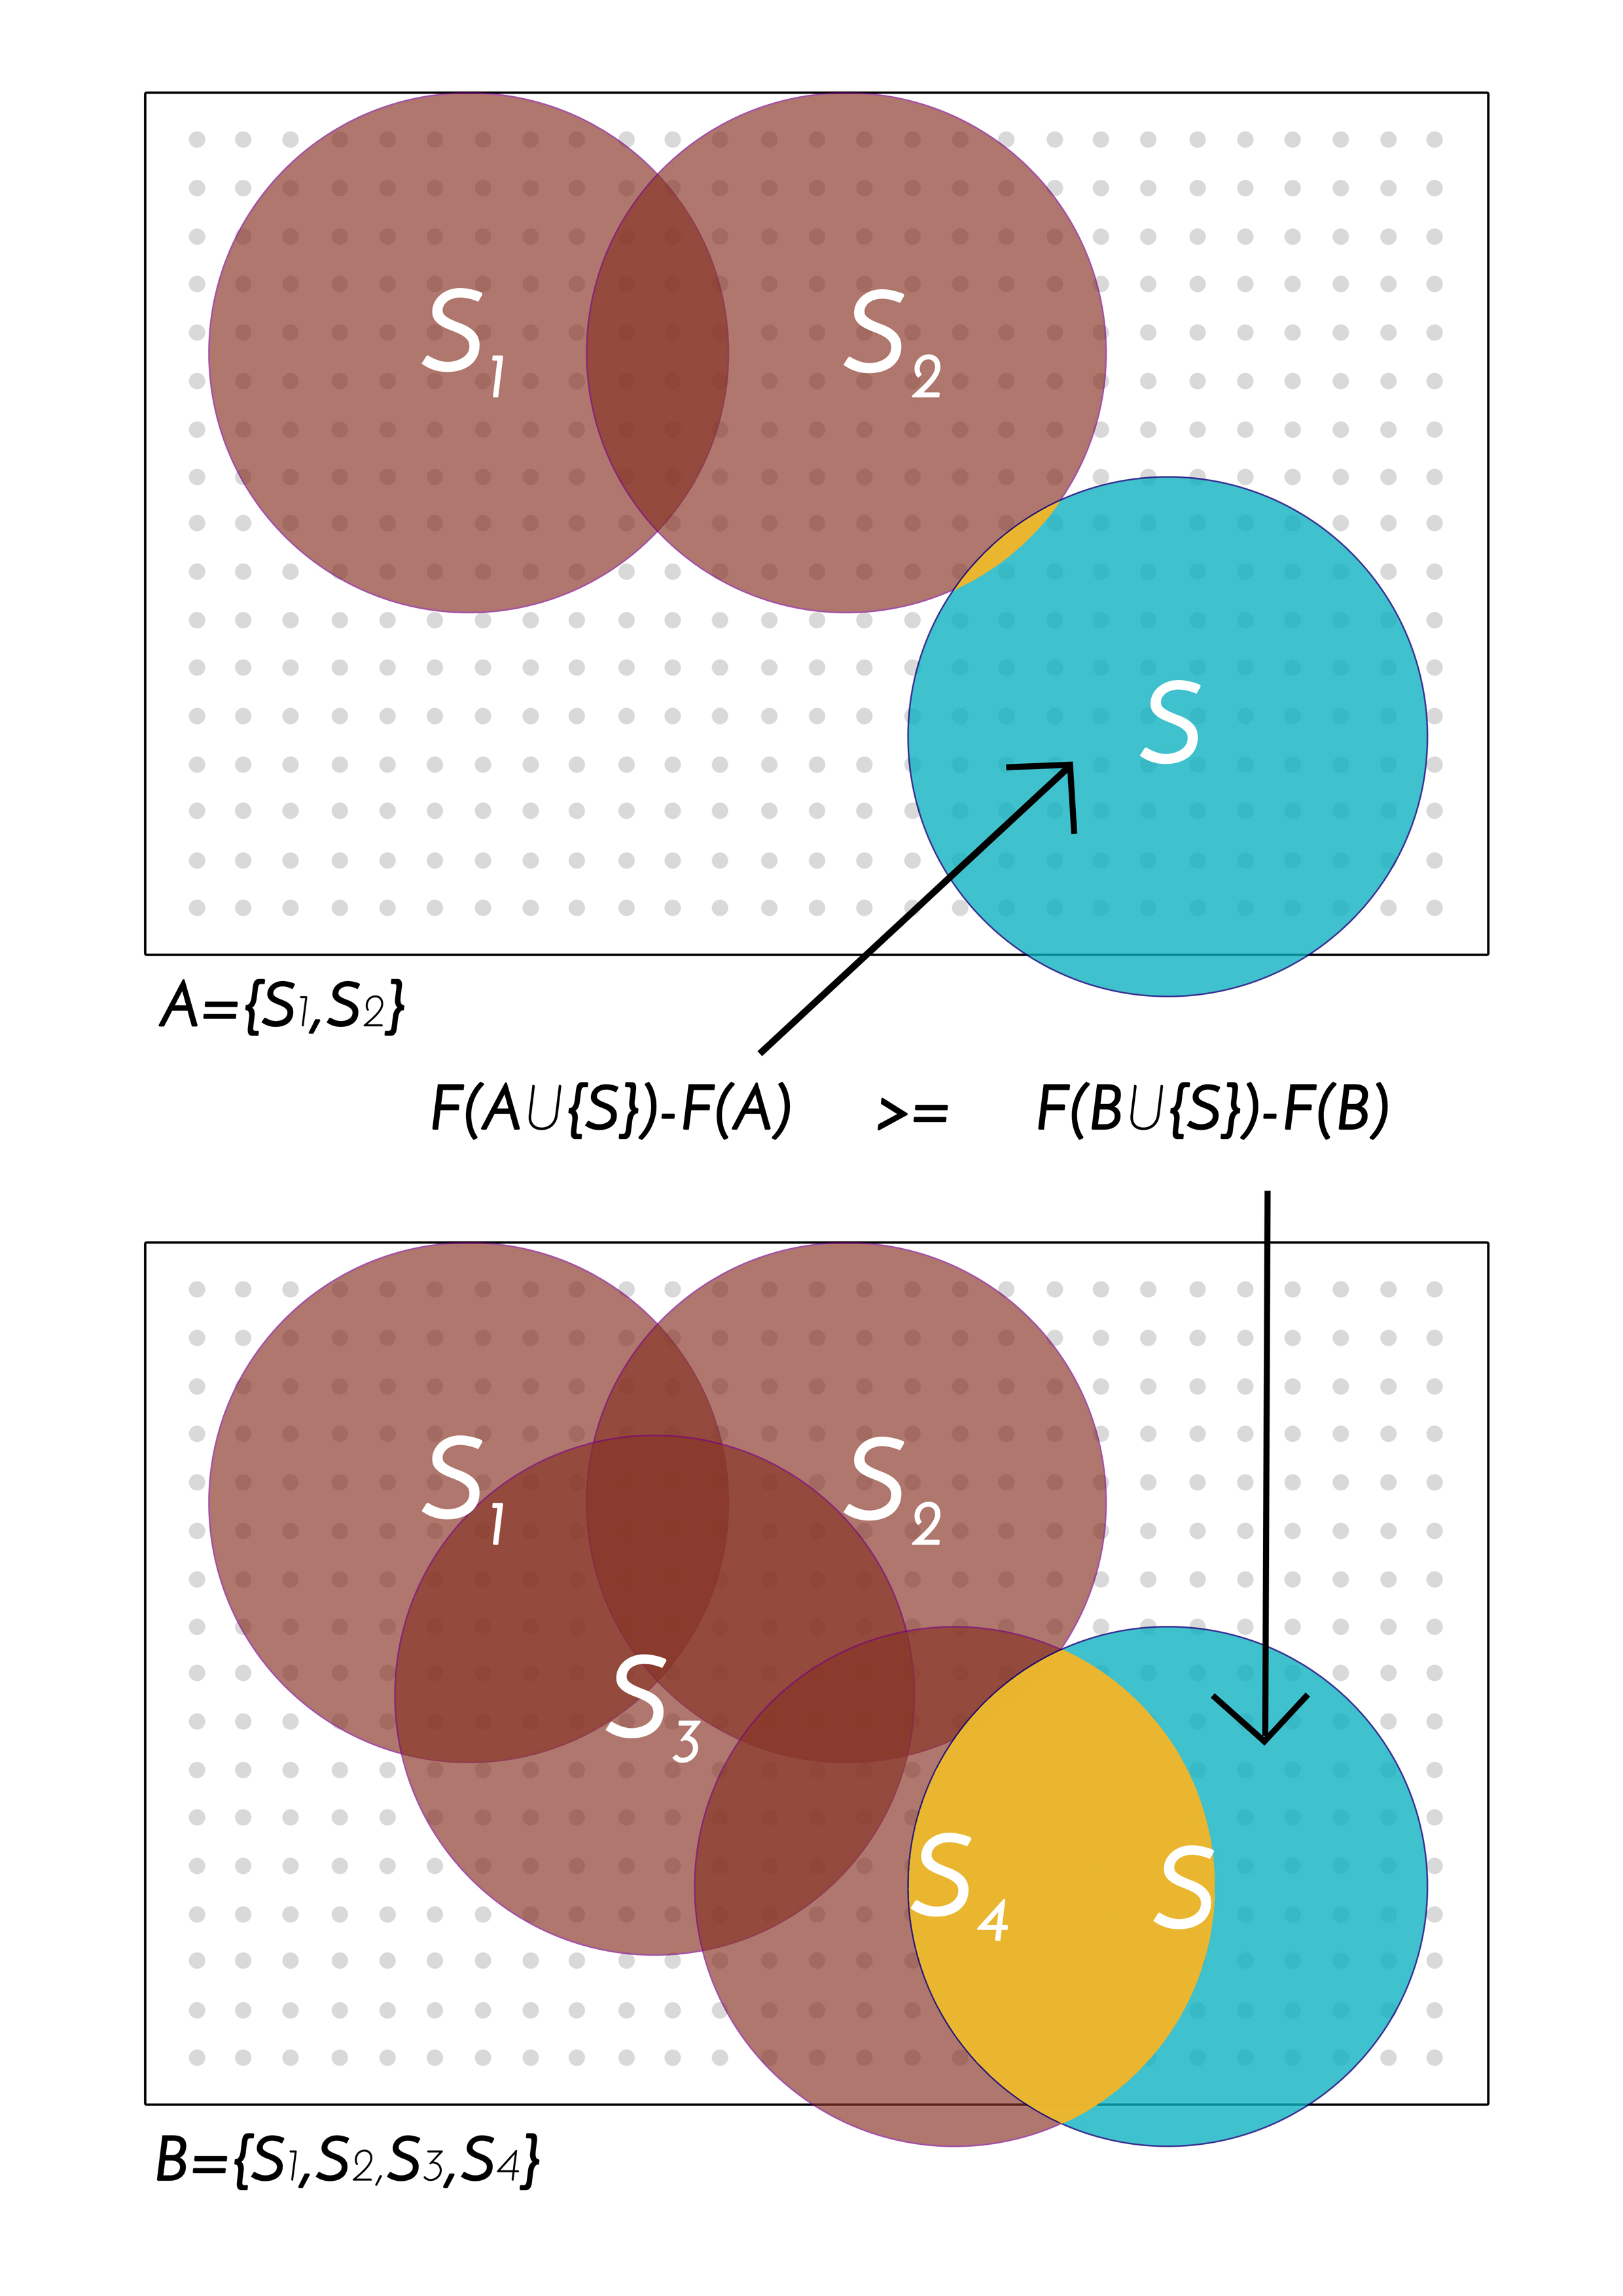
\includegraphics[scale=.25]{./figure_1/figure_1}
	\caption{Submodularity example with sensor placements.}
	\end{center}
\end{figure}

This basically means that submodular functions exhibit a diminishing return property which makes them particularly interesting for optimization. A very intuitive example is the optimum placement of sensors in an area (see figure \ref{fig:submodular}). Sensors can be placed on a grid of locations and function F computes the surface of the space that is being sensed. Note first that adding a new sensor i to the current set S cannot decrease the value of F : $F(S+\{i\})>=F(S)$. Furthermore, if we add sensor i to a small set $S_1$ we tend to get larger improvements than if we add i to a larger set $S_2 \supset S_1$.

Generally speaking, finding the set $ S_k $ of size k that maximizes a set function F is a difficult problem because the number of sets grows exponentially with the number of nodes. Therefore complete enumeration and evaluation is only a feasible solution on very small examples. Nevertheless, if the set function is submodular, a simple greedy heuristic returns a solution $ S_k^{\star} $ such that, in the worst case, $ \frac{F(S_k^{\star})}{F(S_k^{OPT})} \sim 63\%$ (where $ S_k^{OPT}$ is the optimum set of size k) \cite{Krause2014}. This heuristic starts with a set S (possibly empty) and iteratively adds the element i that exhibits the highest marginal gain : $ F(S \cup \{i\}) \geq F(S \cup \{j\})\ \forall j $.

For a ground set of N elements, this heuristic computes F $ \frac{k(2 N - k + 1)}{2} $ times. Since the evaluation of F can be costly, a well-known lazy-greedy variation has been proposed by \cite{Minoux}. This smart implementation uses the submodular structure of the marginal gains in order to reduce the number of calls to F. This requires to maintain a sorted table of marginal gains for all elements. When looking for new element i to add to set S, the top one is selected and the new marginal gain $F(S\cup \{§i\}) - F(S)$ is computed. If this gain is larger than the  gain of the second element in the table, then i is added to S. Otherwise i is inserted back in the table with its updated gain and the same treatment is applied to the element that is now on the top of the table. Because of the submodularity of F, this method performs as well as the original one, but can result in speedups of several order of magnitudes.


\subsection{Gramian based optimization}

Recall that $\mathcal{E}_{min}$ (see eq. \ref{eq:energy}) depends on the initial and final states as well as on the inverse of the gramian matrix W, which only depends on A and B. W can thus be used to obtain information about the average control energy required to move the system in the state space. In the prosumer network that we consider, generators and loads ($\Psi$) are suceptible to change, meaning that initial ($X_0$) and final ($X_f$) states might also vary. In such a scenario, we prefer to aim at good performances on average, rather than very good performances in few specific cases and bad performances in all other situations.

Since the control energy is related to $ W^{-1} $, systems with "large" W will tend to be controlled with low energy. Still, this notion of "large" W is not very accurate and we need to quantify it by taking some metric based on W. We already mentioned the rank of W as being the dimension of the controllable subspace, but it is also known that the trace of W and $W^{-1}$ give information about average controllability and average control energy \cite{Summers2014}. In such a situation, we can build a set function that, given a set of driver nodes S, returns the value of one of these metrics. Indeed, given A and S, we can obtain the system dynamics $(A,B_S)$ and compute the gramian $W_S$. In other word, such a function would quantify the ability of a given set of nodes to contol the system on average.

A key point, demonstrated in \cite{Summers2014}, is that the set function $ F:S \longrightarrow Tr[W_S] $ is modular and the two functions $F:S \longrightarrow Tr[W^{-1}_S] $ ans $ F:S \longrightarrow rank[W_S] $ are submodular. This nice result enables us to look for the driver node set that optimizes some notion of the average controllability using a simple greedy heuristic with a worst case guarantee.

Theoretically, we are now able, for a given prosumer network, to compute A, B, and W. For some trajectory in the state space, we can use equation \ref{eq:ustar} to find the optimum control inputs. However, these inputs do not take into account the physical constraints on the possible trajectories due to lines and batteries finite capacities.

% Considering the dynamic of equation \ref{eq:final_with_control}, we notice that the Gramian based on the transition matrix A is never invertible, meaning that the system should not be controllable. It is easy to see that, indeed, we do not have full control because of the last row of the matrix. Nevertheless, as this row was only added in order to include the power distribution inside A, we do not need to control the system along this "fake" dimension. That is, we only seek the control of the system in the first $ 2N $ dimensions of the space (N phase angles $ \theta_i$ and N frequencies $\omega_i$). Therefore, whenever $ rank[ W(T) ] = 2N$, we will use the Moore-Penrose pseudo inverse of the gramian $ W^\dagger(T) $.

\subsection{Optimization with grid constraints}

\begin{figure}
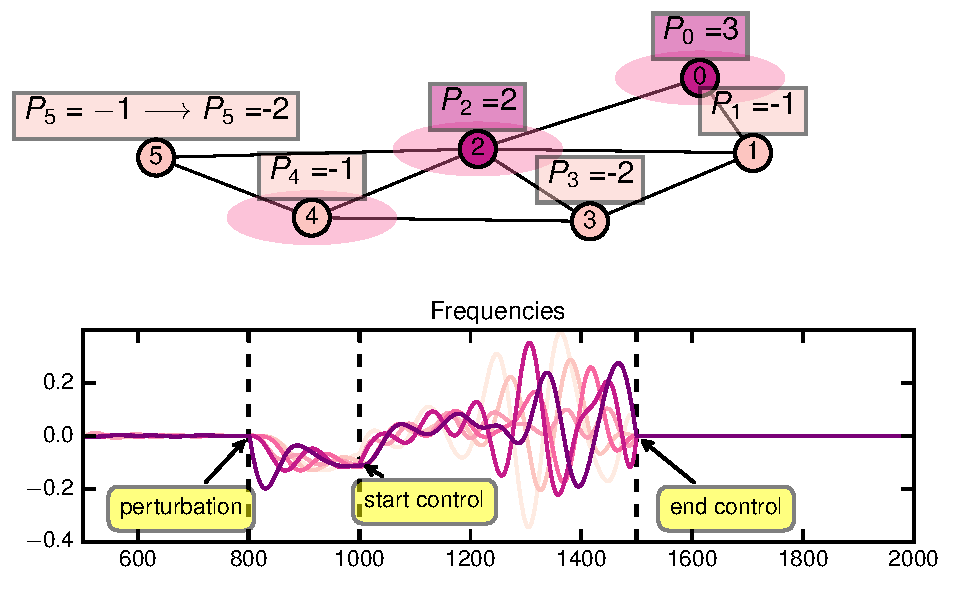
\includegraphics[scale=.55]{plot5.pdf}%./figure_2/figure_2.pdf}
\caption{At $ t_k=800 $, $P_5 $ goes from $-1$ to $-2$ (power inbalance). Consequently, the frequencies $ \dot{ \theta }_i $ deviate from the synchronized state. At $ t_k + d = 1000$, optimal control inputs (see equation \ref{eq:ustar}) are injected at nodes 0, 2, and 4 (nodes with ellipses) such that the system is brought to the synchronized state at time $ t_k + d + T = 1500 $ (T is the control time).} 

%At this time, if the mismatch between production and consumption is still active, we maintain synchrony by using optimal control with $T=1$. }

%Time series of the N frequencies $\omega_i$ (phase angles are not shown for clarity). $d$ is the delay between the perturbation and the begining of the control phase that bring the system bak in the synchronized state in T time steps. Here, $d$ was chosen quite large for the clarity of the figure. Note that, if the perturbation is still active at this point, the system still needs control in order to stay synchronized (batteries should still compensate the power imbalance)}
\label{fig:frequecies}
\end{figure}

Finding the driver set $S_k$ of size k using the gramian $W_{S_k}$ of the system $(A,B_{S_k})$ does not require initial and final states. Besides, $W_{S_k}$ does not depend on the modified power distribution $ \Psi $ of the nodes. We are indeed looking for k controllers that perform well on average over all possible situations. On the contrary, the constraints derived above (eq. \ref{eq:flow_cons}, \ref{synchro_constraint}, \ref{level_constraints} and \ref{rate_constraints}) are bounded to a particular trajectory in the state space. We indeed check wether the power grid can sustain the controlled dynamics when transitioning from a given initial state to a target final state. As we do not know what these states could be, we could use multiple scenarios and test wether $S_k$ can control the system without violation of constraints. In this paper, we use a slightly different approach. We consider that the system is initially at equilibrium (all elements are synchronized at $\Omega$) and that control will be necessary if a perturbation (power inbalance) occurs and takes the system out of equilibrium (see figure \ref{fig:frequecies}). Depending on how much time we need to start the control phase, the state of the system (the initial state for control) might be "somewhere around" the synchronized state. In order to test wether a set $S_k$ can control the system without violation of constraints, we sample initial states within some hypersphere centered on the synchronized state and check all the constraints. If for all trajectories, the constraints are respected, then we consider that $S_k$ enables the control of the system.

Increasing k means that we deploy more strorage which increases the costs but tends to lower the energy required as we will see in the next section. Using the submodularity of the set functions introduced above, we can build a sequence of growing sets $S_1 \subset S_2 \subset ... \subset S_k $ and stop as soon as $S_k$ enables the control of the system for some k.

%We propose the following greedy algorithm in order to find the smallest set of locations that minimizes the average control energy and satisfy the constraints. We assume here that the system is in a given initial state $ Y_0 $ and we want to reach a desired final state $ Y_f$  in $ T $ time steps. The algorithm \ref{algo_1} starts with an empty set and, as long as that constraints are not satisfied, it increases the size of the set. For a given size k, the set $ S_k $ is found using lazy greedy submodular optimization of a Gramian-based set function F. In practice we use $ F(S) = -Tr \left[ W_S^{\dagger}(T) \right] $ which quantifies the average energy required to move the system around the controllable subspace. The algorithm \ref{algo_1} returns then the tuple $ (k,S_k,u^{\star}) $ such that $ S_k $ is the smallest set that minimizes the average control energy and, in this case, satisfies the constraints with control $u^{\star}$. 

\begin{algorithm}
	\begin{algorithmic}
				\State $k=0$
				\State $S_k = \emptyset $
                \While{ Not Constrained control}
                	\State $k \gets k+1$
                	\State $ S_k = S_{k-1} \cup argmax_{i \in N \setminus S_{k-1} } F(S_{k-1} \cup \{i\}) $
                \EndWhile
     \end{algorithmic}
     \caption{Optimization with grid constraints}
        \label{algo_1}
\end{algorithm}

%\begin{algorithm}
%        \begin{algorithmic}
%                \While{  \small $ Not\ \left\{ \begin{array}{lll} 
%                                              rank \left[ W_{S_k}(T) \right] < 2N\ and \\ 
%                                              \forall t,\forall (i,j) \in V^2, g_{ij} \left| \theta_j(t) - \theta_i(t) \right| \leq 1\  and \\
%                                              \forall t,-\frac{\Lambda(0)}{I \Omega} \leq -\sum_{k=0}^{t}u^{\star}(k) \leq \frac{ \Lambda_{MAX} - \Lambda(0)}{I \Omega}and \\ 
%                                              \forall t,\ \left| u^{\star}(t) \right| \leq \frac{r}{I\Omega}
%                                              
%                                              \end{array} 
%                                              \right. $ }
%    \State $k\ \ \ \ \ \ \ \ \ \ \ \gets k+1$
%    \State $ S_k \ \ \ \ \ \ \ \ \ \gets Subopt(F, k)$
%    \State $ u^{\star}(t)\ \ \ \ \ \ \gets OptControl( S_{k} )$ 
%\EndWhile
%        \end{algorithmic}
%        \caption{Greedy submodular optimization with constraints}
%        \label{algo_1}
%\end{algorithm}
\normalsize



\section{Results}
\label{sec:Results}

%We first consider a small example of 10 nodes connected with an erdos-renyi topology. The power distribution and the capacities of the lines are selected randomly such that the system is at equilibrium. Therefore, the production matches the consumption, no line is overloaded and all nodes are synchronized to the main frequency. We use the greedy algorithm \ref{algo_1} based on the trace of the inverse Gramian as to select the driver set $S$. At a given time $ t_k $, we introduce a small perturbation in the form of a mismatch between the production and consumption : $P_i(t_k) = P_i(t_{k-1}) + \delta P$ for some random node i. Consequently, the frequencies $ \dot{ \theta }_i \forall i $ of the oscillators start to deviate from the synchronized state. At time $ t_k + d $, we apply to the drivers the optimal control of equation \ref{eq:ustar} such that the system is brought to the synchronized state at time $ t_k + d + T $, where T is the control time. At this time, if the mismatch between production and consumption is still active, we maintain synchrony by using optimal control with $T=1$. Figure \ref{fig:frequecies} shows the evolution of the nodes' frequencies during the control phase.



The purpose of selecting the drivers according to a Gramian related metric is to minimize, on average, the amount of control energy needed. Conversely, if we select the drivers randomly, we expect to need, on average, more energy to control the system. In figure \ref{fig:densities}, we compare the average control energy  $log(\mathcal{E})$ in function of the proportion of drivers amoung the total number of nodes $n_D = N_D/N_{nodes}$, for a set of drivers selected thanks to our algorithm with randomly selected drivers (in both cases overloading and battery limits constraints are satisfied). We draw $10^4$ scale-free topologies with 50 nodes, and random power distributions and line capacities.  For each system we select a random number of drivers $N_D \sim \mathcal{U}(1,N_{nodes}) $ and we find two driver sets of size $N_D $. One is chosen randomly and the other is found with algorithm \ref{algo_1}. For both sets, if the control is possible, we draw a random initial state $Y_i$ and a random final state $Y_f$, and we compute the control energy required for driving the system from $Y_i$ to $Y_f$. Since the algorithm is based on $ Tr[W^{-1}]$, we could plot $ Tr[W^{-1}]$ in function of $n_D$ but we prefer to validate our method by computing the actual average energy. As expected, both curves decrease as the number of drivers increases, meaning that, as the number of drivers grows, the average control energy tends to decrease, but we tend to use less energy when the drivers are selected with our algorithm. Note that this difference tends to zero when $n_D$ tends to one, because almost all nodes are then selected, yielding little flexibility for optimization.

%For each system we find the driver set S using algorithm (X) and we draw a random driver set $S'$ such that $S$ and $S'$ have the same size, and such that $S'$ also provide full control of the system. We then compute the control signals and the corresponding control energies $\mathcal{E}_S$ and $\mathcal{E}_{S'}$ for both $S$ and $S'$. Each system can therefore be represented as a point with coordinates $(|S|, \mathcal{E}_S)$. On figure 2, we plot the densities of these points for the random case (left pannel) and the optimized case (right pannel). Regions in dark red contains a lot of points while regions in dark blue have very few points. Figure 2 shows that most of the systems considered tend to be controlled by the drivers of algorithm X with less energy and/or drivers than for the random case.


\begin{figure}
\includegraphics[scale=.55]{plot4.png}%./figure_3/figure_3}
\caption{$log(\mathcal{E})$ against $n_D$ for random and optimized driver sets ($ N_{nodes} = 50 $).}
\label{fig:densities}
\end{figure}

We investigate next how the topology of the grid and the physical constraints affect the minimum size of the driver set. The driver set size $n_D$ is no longer selected randomly, but minimized. We consider the simple case of an Erdös-Rényi topology with probability of connection p. We show on Figure \ref{fig:erdos_renyi} how the minimum size of the driver set evolves with p for different Gramian based metrics and for two levels of constraints : 

\begin{itemize}
\item Level 1 : full control and grid constraints (see section \ref{sec:The_Model}). The system is controllable (i.e it can be moved from any point to any other point) and under the constraints (i.e it can be moved without overloading any line or breaking any battery limits).
\item Level 2 : full control only : the system can be moved from any point to any other point of the state space, without considering any overloading or battery limit constraints. 
\end{itemize}

\begin{figure}
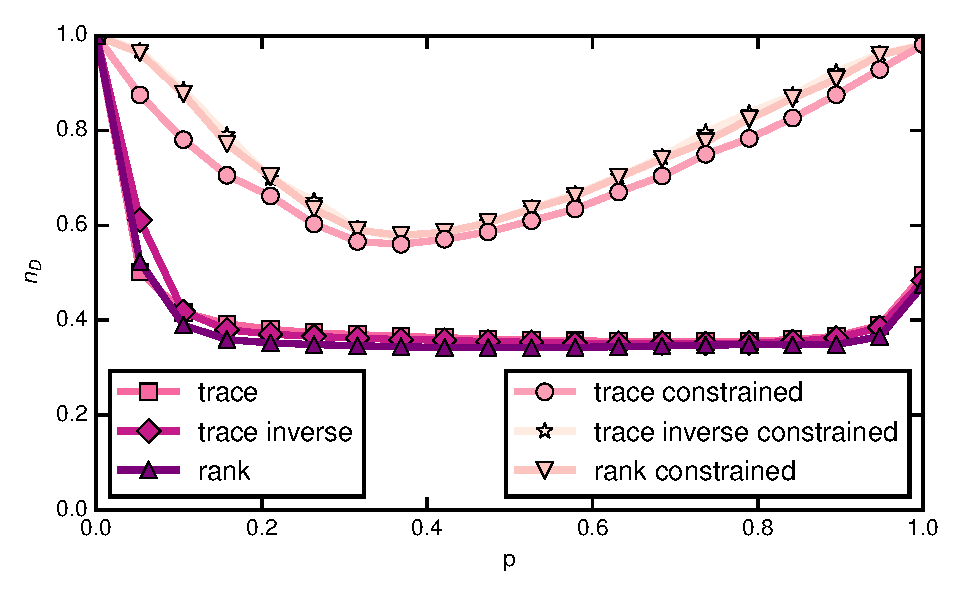
\includegraphics[scale=.55]{plot3.pdf}%./figure_4/figure_4}
\caption{ $ n_D $ against link probability p for erdos-renyi topologies ($ N=100 $). Curves are averaged over 100 realizations. The top three curves show the results for the three metrics taken into consideration when all constraints are considered (see Level 1 in the main text). The bottom three curves exhibit the results for the same metrics when only the full controllability constraint is considered (see Level 2).}
\label{fig:erdos_renyi}
\end{figure}


When $p \sim 0$, nodes tend to be very poorly connected such that we need to control almost all nodes in the grid. As p increases, the connectivity of the graph rises and the number of drivers decreases. At some point, the connectivity of the graph starts to harm its controllability, and more drivers are needed (this effect is in accordance with the litterature). As expected, the driver sets for the level 1 of constraints are larger than for level 2 (for all metrics) because we impose far more constraints on the control inputs.



%Because transmission power grids are spatially constrained (each contry has its own transmission grid which is interconnected with neighboring grids at some specific locations), we study the control in clustered graphs. More precisely, we use a block model $(N, N_{clusters}, p_{in}, p_{out} ) $ to generate random topologies where $ N $ is the number of nodes, $N_{clusters} $ is the number of clusters, $p_{in} $ is the probability that two nodes within the same cluster are linked, and $ p_{out} $ is the probability that two nodes in two distinct clusters are connected.
%
%
%\begin{figure*}
%	\begin{center}
%		\includegraphics[scale=.5]{Blockmodel.png}
%		\caption{left panel : $n_D$ against $N_{clusters} $ for different values of $ p_{in} $ and $ p_{out} = 0.1 $. $ N=200 $ and curves are averaged over 100 realizations. right panel : $n_D$ against $ p_{in} $ for systems of $N=200 $, $p_{out} = 0.1 $, and for different values of $N_{clusters} $. The curves are averaged over 100 realizations.}
%	\end{center}
%\end{figure*}
%
%%\begin{figure}
%%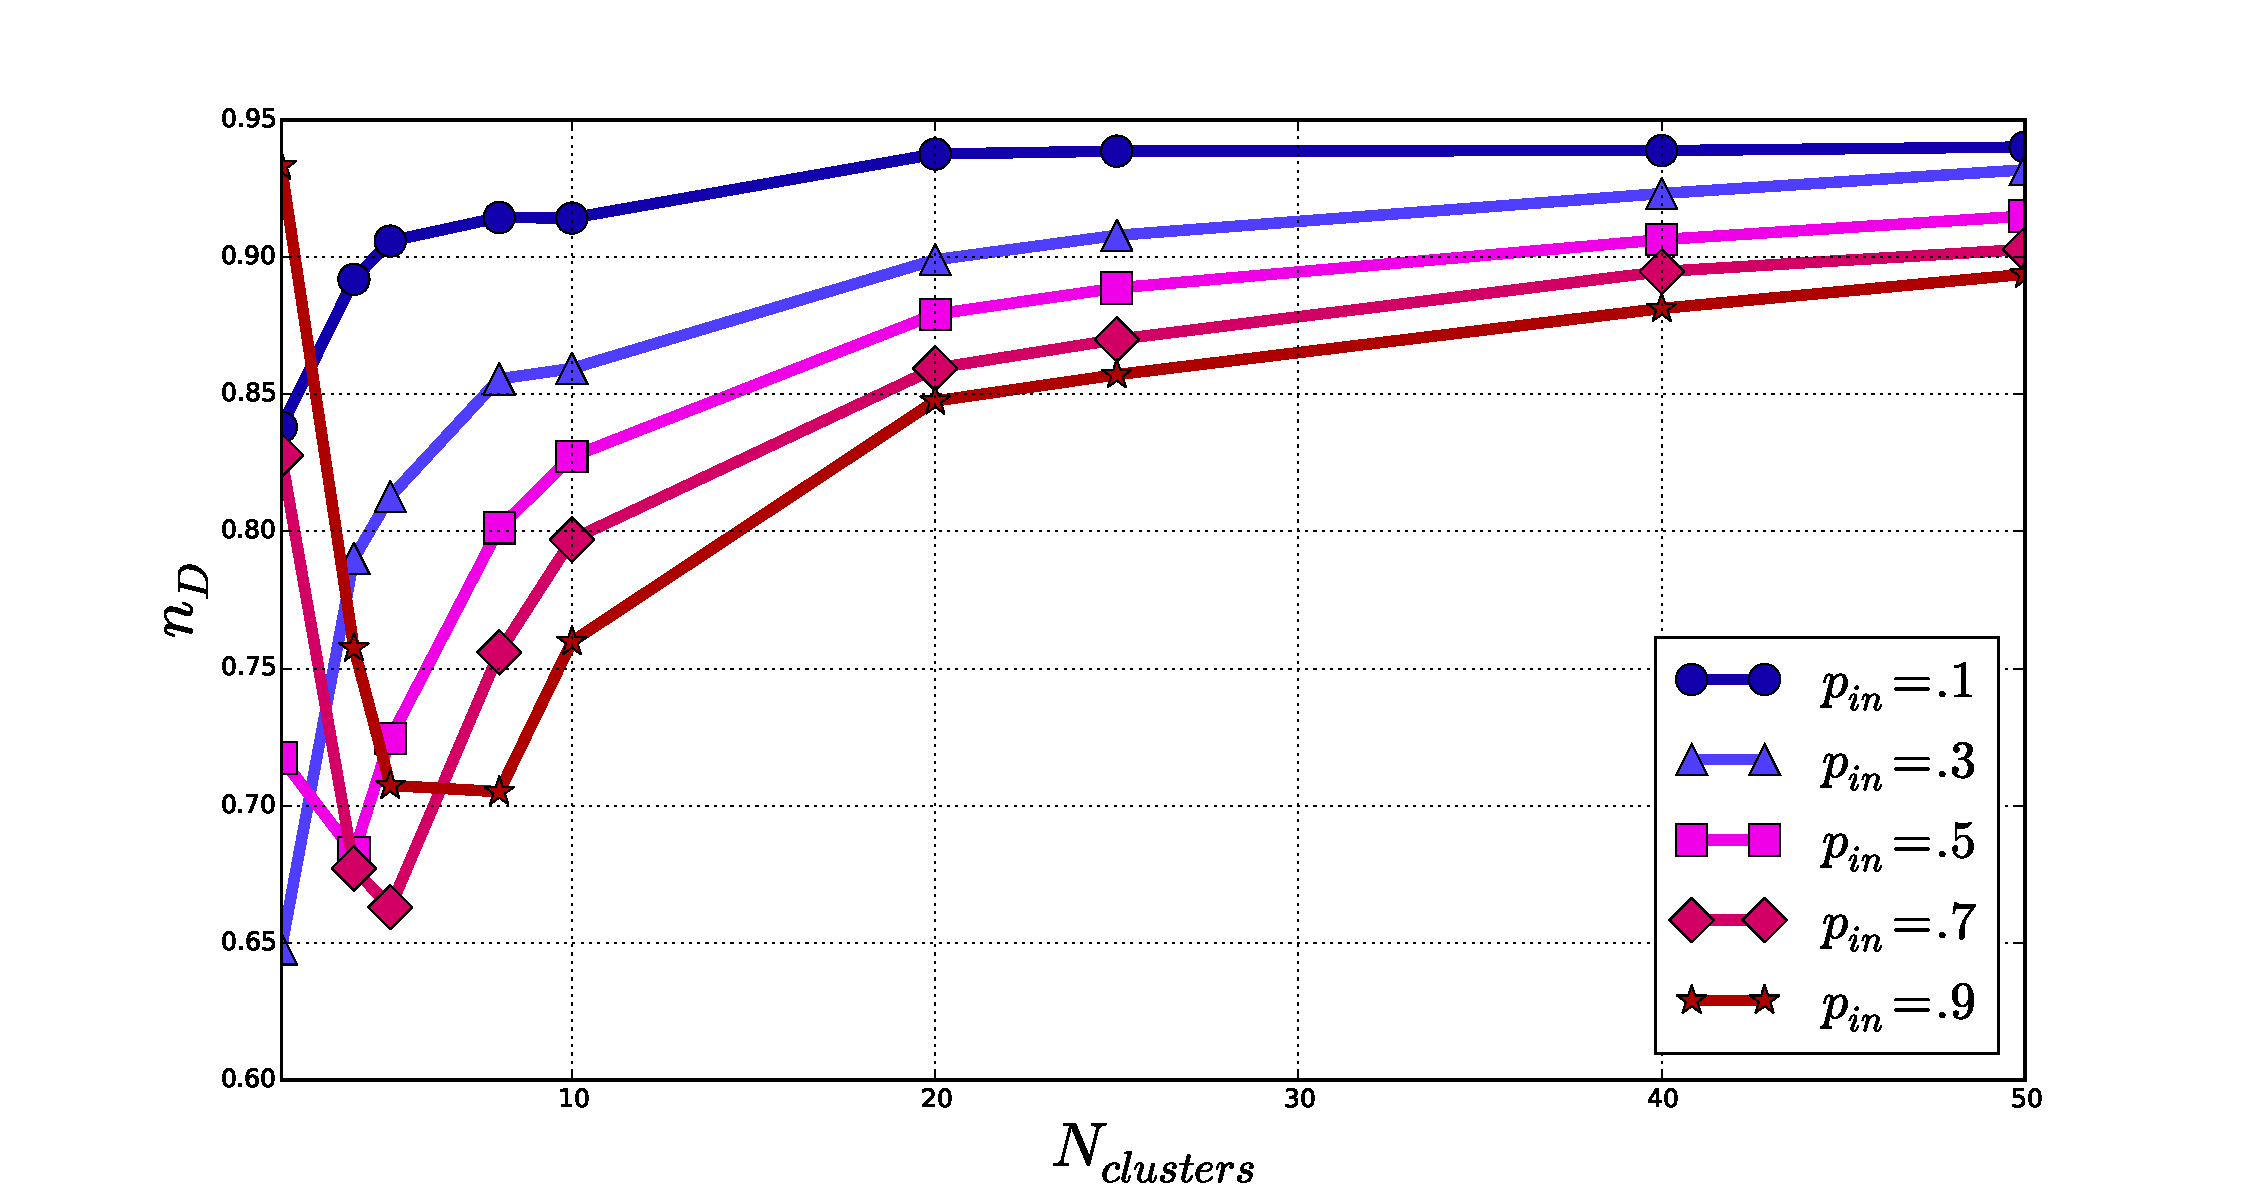
\includegraphics[scale=.25]{./figure_5/figure_5}
%%\caption{$n_D$ against $N_{clusters} $ for different values of $ p_{in} $ and $ p_{out} = 0.1 $. $ N=200 $ and curves are averaged over 100 realizations.}
%%\label{fig:block_model_1}
%%\end{figure}
%
%
%Figure \ref{fig:block_model_1} displays how the number of drivers evolves with the number of clusters for different values of $ p_{in} $ when $ p_{out} $ is fixed ($p_{out} =0.1$). For small values of $ p_{in} \sim p_{out} $ clusters are poorly marked, and the connectivity is low. The number of drivers in these conditions is large and increases slowly when the number of clusters augments. As $ p_{in} $ increases, the clusters becomes more densily connected such that within a cluster less drivers are required in order to control it. As the number of clusters grows, more drivers are required. For large values of $p_{in} $, the behavious is more complex. We see indeed that for $p_{in} = 0.9 $ and $N_{clusters} = 2$, almost $ 94\% $ of the nodes are needed for control, but this quantity first decreases with the addition of a few more clusters ($ 71\% $ for $ N_{clusters}=5 $), before increasing. This behavior can be explained by the fact that controlling a very dense network requires, in our settings, a very large portion of nodes to be drivers. Controlling one cluster alone thus requires to control almost all nodes within this cluster. Nevertheless, when a relatively small (compared to the number of nodes in the graph) number of clusters are interconnected with a few links, nodes in one cluster are able to control nodes in other clusters to which they are connected. As the number of clusters grows, the global connectivity increases rapidely, such that the number of drivers also rises. We show this behavior in more details in figure \ref{fig:block_model_2}, where the number of drivers is plotted against $ p_{in} $ for $N=200$ and $N_{clusters} \in \{2,4,5,10\} $. For $N_{clusters} = 2 $ and $ p_{in} = 0.1 $ the number of drivers is large since the graph is poorly connected. When $p_{in} $ increases, $n_D$ decreases until a minimum value $n_D \sim 0.6 $ at $ p_{in} \sim 0.25 $. After this point, $n_D$ augments with $p_{in}$. For $N_{clusters} = 10 $, we do not see this behavior : $ n_D $ decreases continuously as $p_{in} $ increases as expected from the curves of figure \ref{fig:block_model_1}.
%
%
%%\begin{figure}
%%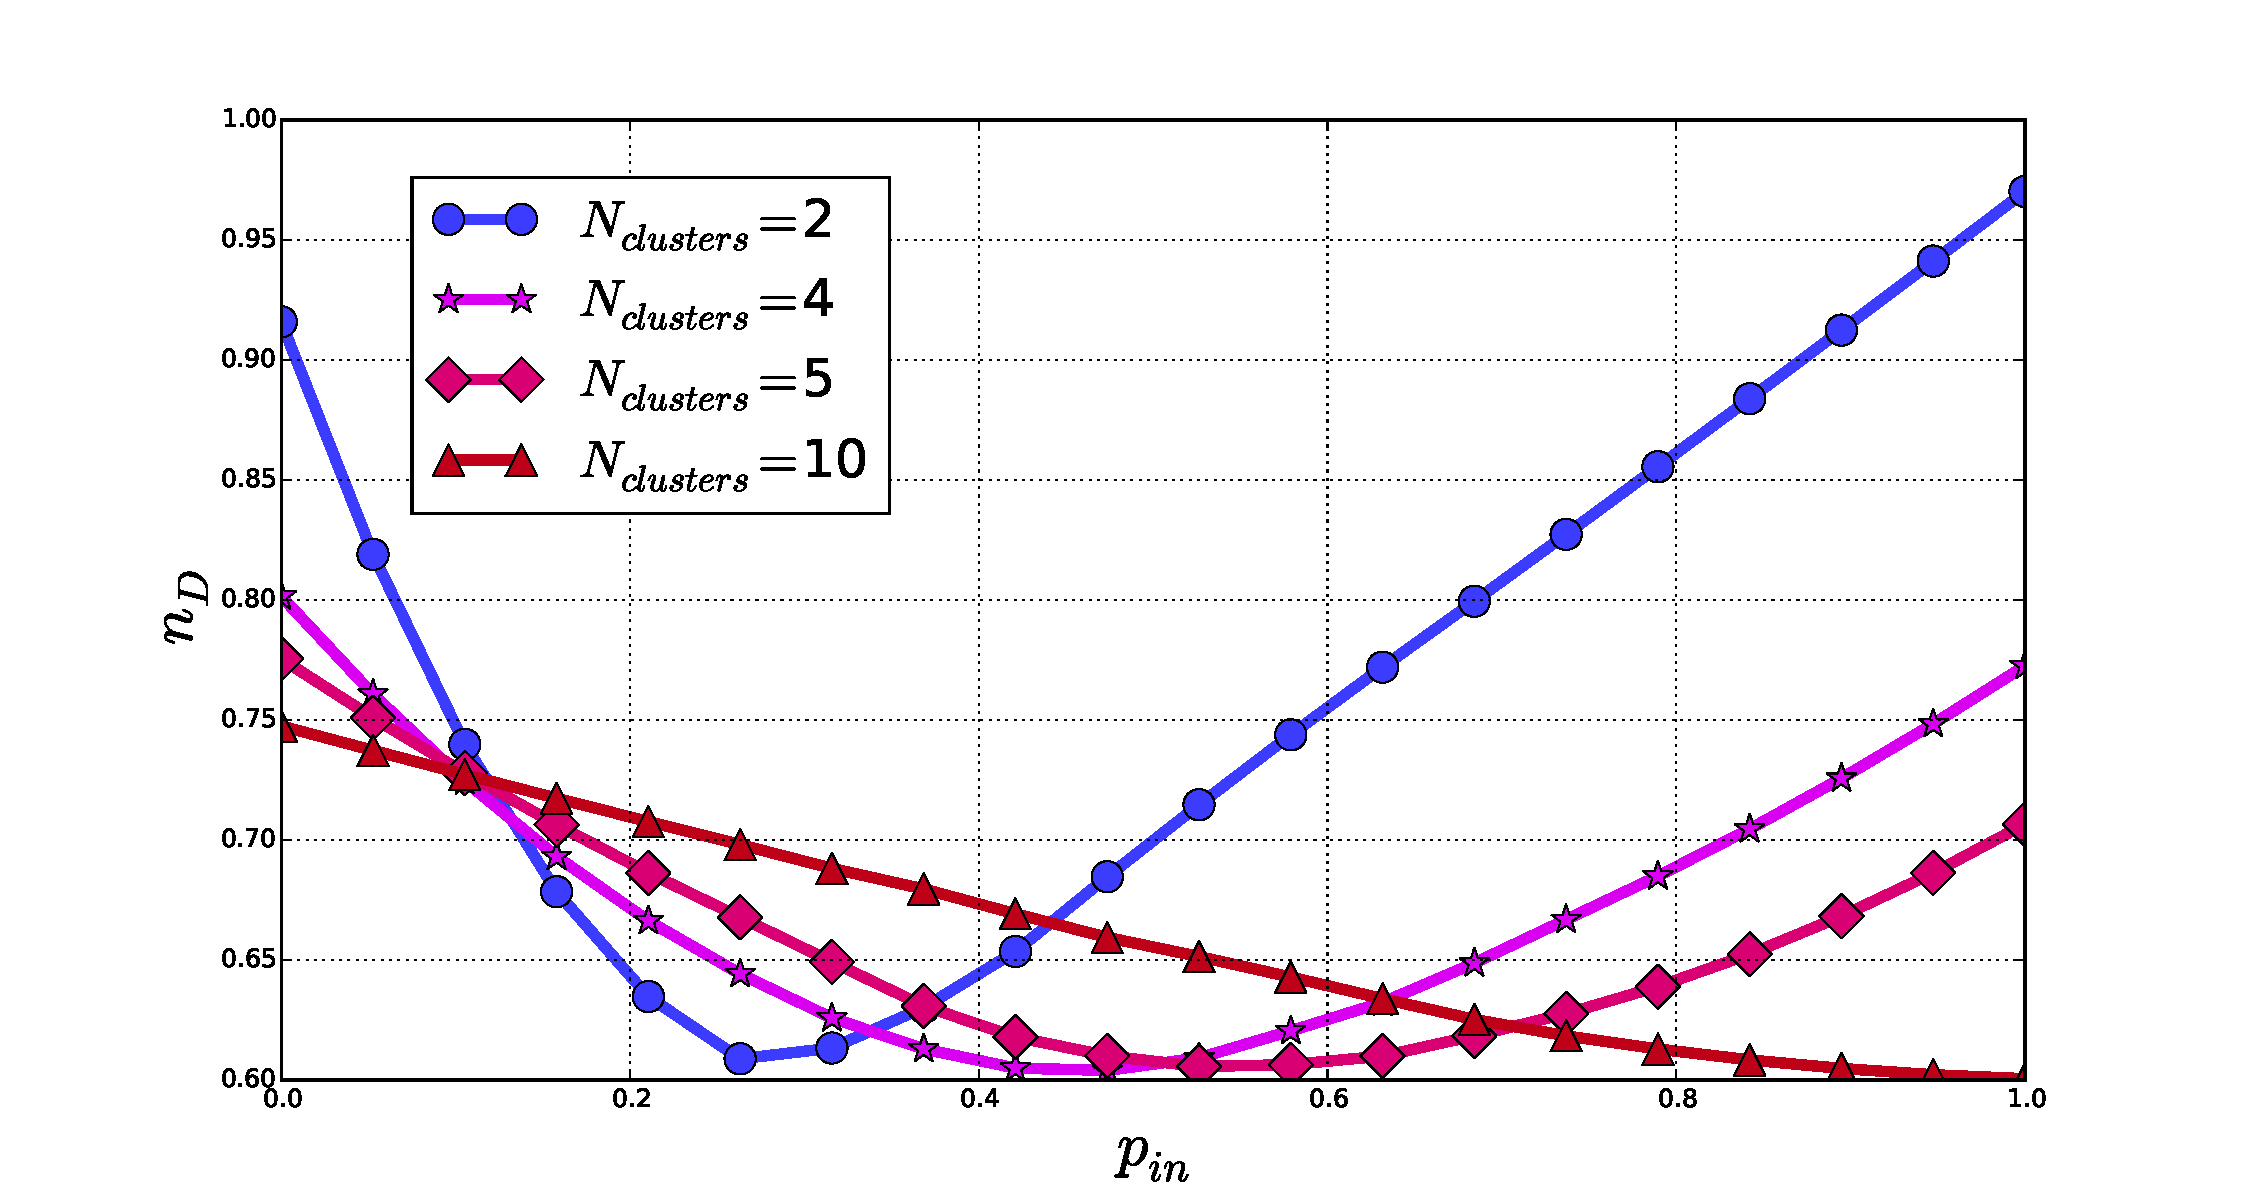
\includegraphics[scale=.25]{./figure_6/figure_6}
%%\caption{$n_D$ against $ p_{in} $ for systems of $N=200 $, $p_{out} = 0.1 $, and for different values of $N_{clusters} $. The curves are averaged over 100 realizations.}
%%\label{fig:block_model_2}
%%\end{figure}
%
%
%Until now, we have considered all batteries to be equal, i.e they have the same capacity and charge/discharge rate. Although simple, this assumption might not be verified in practice where different types of batteries exist. Optimizing the locations of different types of storage as to optimize the cost / reliability tradeoff is out of the scope of this paper. Nevertheless, we studied how the number of drivers behaves when the batteries have different capacities. More precisely, we draw the capacities of the batteries from a normal distribution $ \mathcal{N}( \mu_{\lambda}, \sigma_{\lambda} ) $ and keep a simple erdos-renyi topology for the power grid. Note that each node is assigned a capacity regardless of its caracteristics (degree, betweeness, and so on...). In figure 6, we plot $n_D$ as a function of the relative standard deviation of the battery capacity distribution $ \sigma_{\lambda} / \mu_{\lambda} $. We see that $n_D$ increases with the variance of the capacity distribution for all three gramian based metrics considered. Moreover, this rise is abrupt since $n_D$ goes from $ 60 \%$ for $\frac{\sigma_{\lambda}}{\mu_{\lambda}} \sim 0.15 $ to $100 \% $ for $\frac{\sigma_{\lambda}}{\mu_{\lambda}} \sim 0.27 $. 
%
%\begin{figure}
%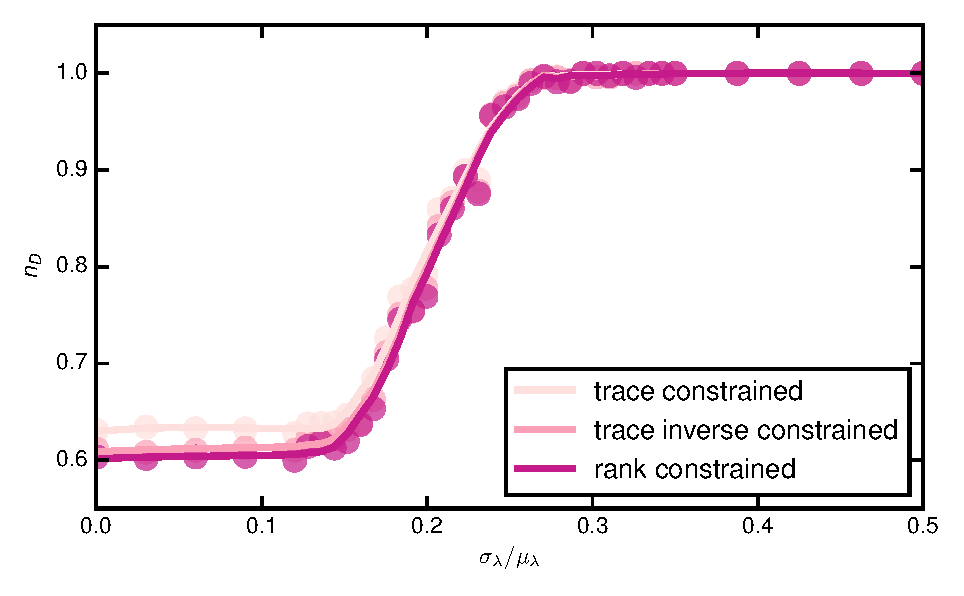
\includegraphics[scale=.55]{plot2.pdf}%./figure_7/figure_7}
%\caption{$n_D$ against the relative standard deviation of the capacity distribution of the batteries $ \frac{ \sigma_{ \lambda } }{ \mu_{ \lambda} } $. The dots are averages over 100 realizations and the curves are obtained using a Savitzky-Golay filter, each color shows the results for a given metric. The graphs are erdos-renyi with $N=100$ and $p=0.3$, and $\mu_{\lambda} = 100 $ units. }
%\label{fig:batteries_variance}
%\end{figure} 
%
%\begin{figure}
%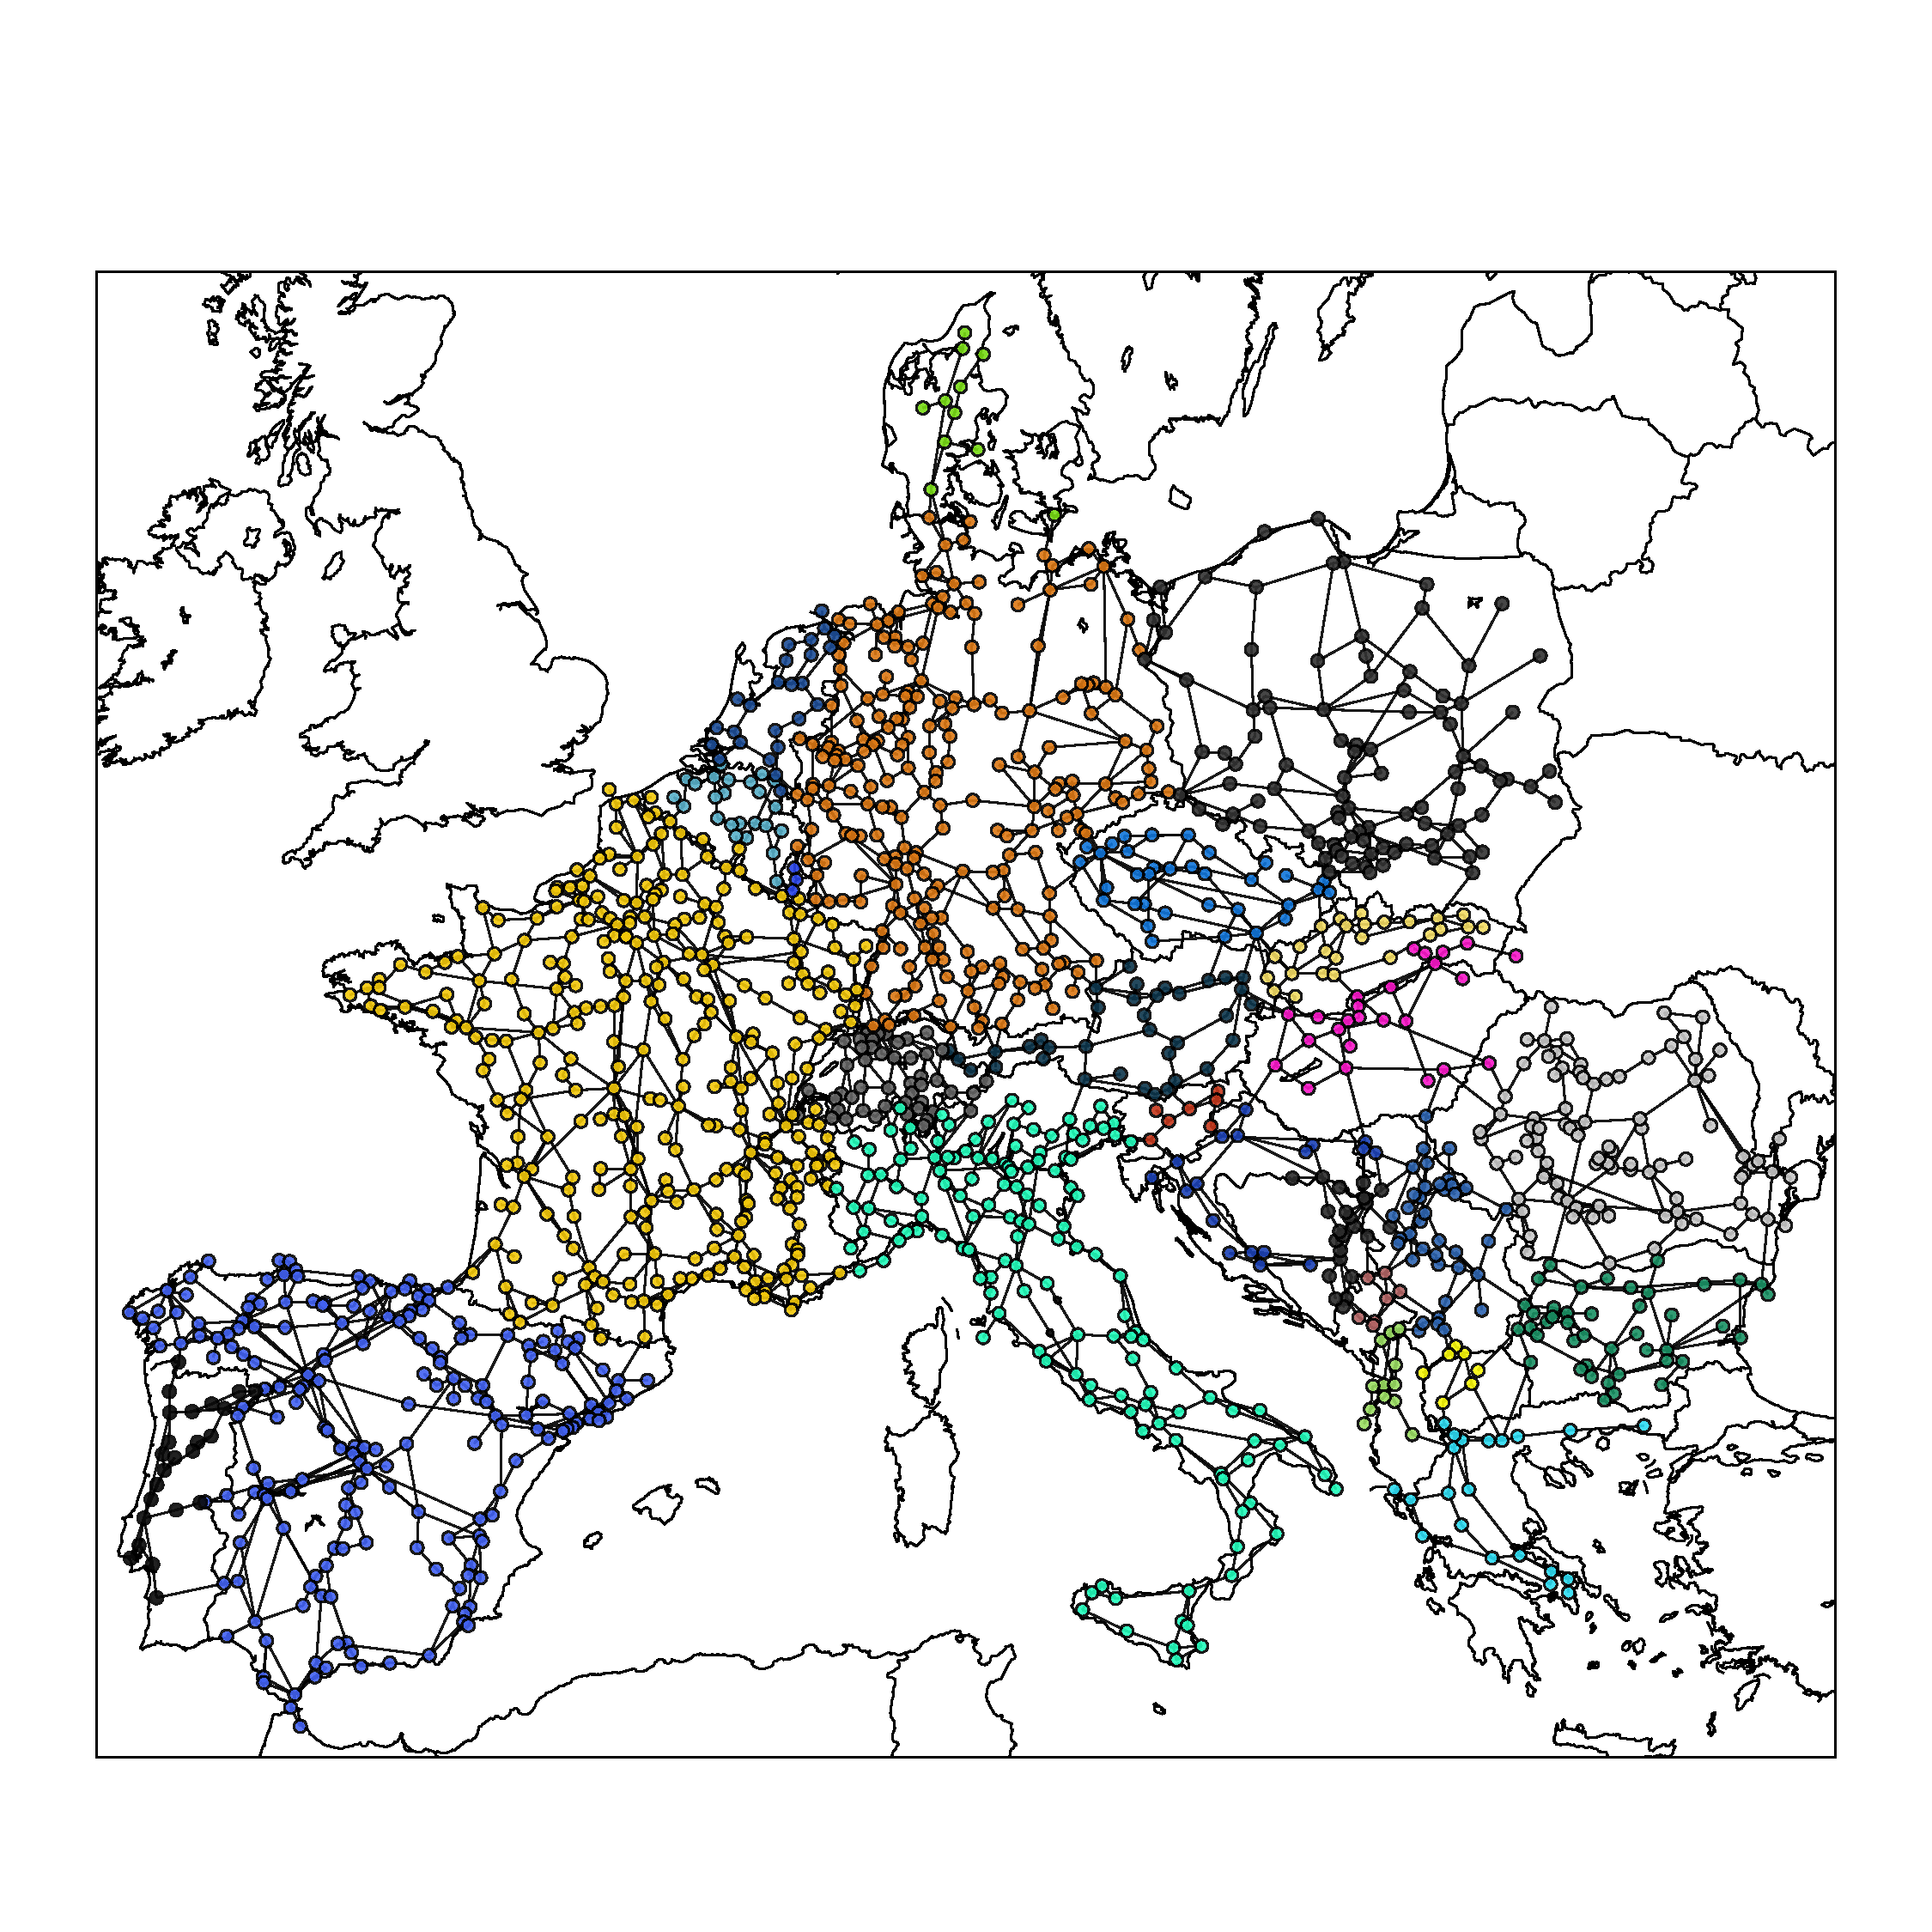
\includegraphics[scale=.25]{power_grid}
%\caption{European transmission power grid \cite{jensen_2015_35177}. Nodes are colored according to their county.}
%\label{fig:network}
%\end{figure}
%
%Since real power grids topologies are known to be far from random, we consider here, as a real case, the european transmission power grid which topology was obtained from \cite{jensen_2015_35177}. The network contains 1494 nodes and 2156 edges and spans 25 european countries. A representation of this graph can be found in figure \ref{fig:network} where the nodes are colored according to their country. We select the power distribution and the line capacities randomly, and use the method described above.
%
%We use the trace of the Gramian matrix for the optimization. The top panel of figure \ref{fig:real_case} shows that the rank of the Gramian increases with the size of the controllers until reaching full rank ($rank[W_S] = 2 N_{nodes}$) for $N_D=1244$. Above this point, we compute the average control energy needed to drive the system from an initial random state to a random final state. The curves on the bottom panel of figure \ref{fig:real_case} show the results for the optimized driver sets and for random driver sets. As can be seen on figure \ref{fig:real_case}, as the size of the driver set increases, the control energy tend to decrease. But, we need less energy with the optimized driver set than with randomly sampled sets.   
%
%\begin{figure}
%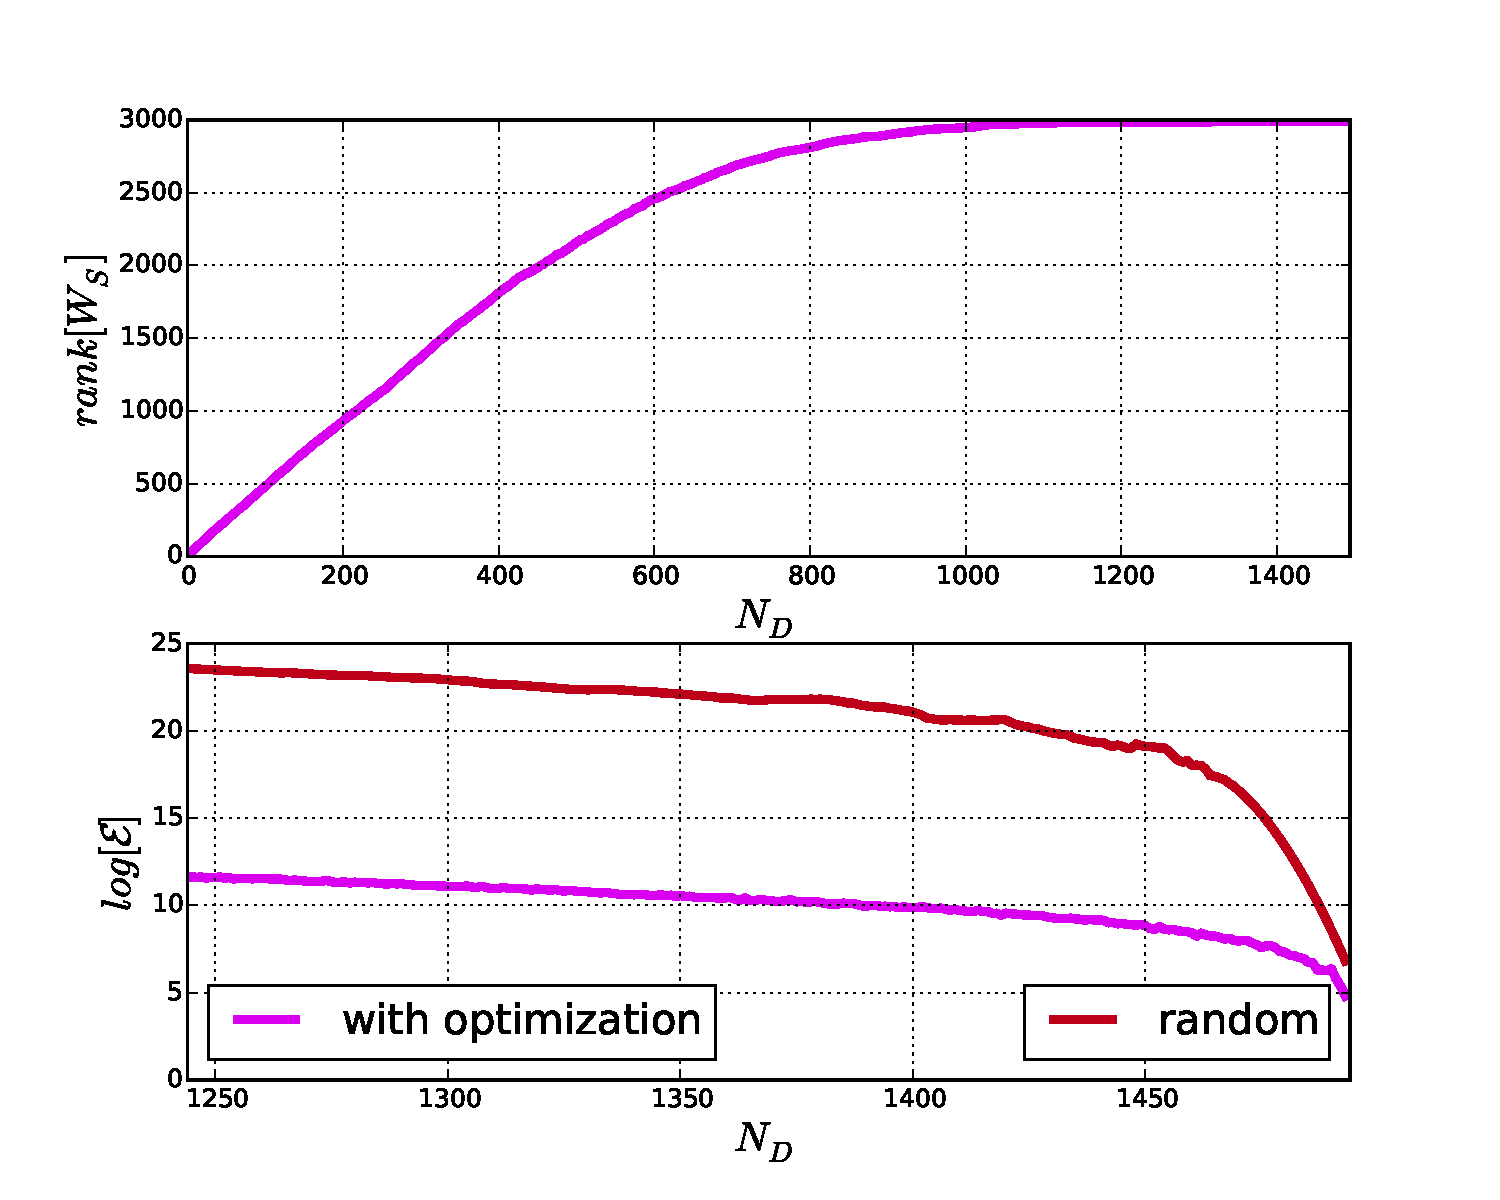
\includegraphics[scale=.4]{figs2}
%\caption{Gramian rank and control energy evolution for european transmission power grid (see figure \ref{fig:network}).}
%\label{fig:real_case}
%\end{figure}
%%In this section, we provide some results in order to illustrate the work described above. We use a small 10 prosumers example, connected with a random topology. The line maximum capacities are selected  according to a normal distribution $\mathcal{N}(\mu_l,\sigma_l)$.  The power distribution is chosen as a zero mean normal distribution $ \mathcal{N}(0,\sigma_p) $, and the samples should satisfy the constraints \ref{synchro_constraint} and \ref{zero_sum_constraint}. Obviously, $\mu_l$, $\sigma_l$, and $\sigma_p$ should be chosen such that, without any perturbation, the lines are not already overloaded.
%
%%Once the synchronized state is reached, we apply a perturbation to the power distribution such that there is a mismatch between production and demand (constraint \ref{zero_sum_constraint} is not satisfied). We denote by $d$ the delay between the perturbation and the start of the control phase (see figure \ref{fig:frequecies}). $d$ depends on how fast the perturbation can be identified and located, the control inputs calculated and communicated without error through the communication network.
%
%%If the driver set is fixed, we expect that the higher $ d$, the higher the control energy required to drive the system back to the synchronized state. Eventually, if $d$ is too large, the minimum energy control inputs will result in some constraints being broken (battery levels, line flows, and so on...).
%
%%As visible on figure \ref{fig:energy_vs_delay}, when d increases, the system deviates more from the equilibrium and this results in more energy being used to steer it back to synchrony. We also investigate here how the driver node set selected with algorithm \ref{algo_1} performs against other driver sets of the same size. we use a Monte-Carlo sampling of the drivers sets of the same size as our solution, and filter out the ones that do not meet all the constraints. Figure \ref{fig:energy_vs_delay} shows that our solution (blue dotted curve) uses less energy than other driver sets of the same size (red curve).


\section{Conclusion}
\label{sec:Conclusion}
In this paper, we considered the case of networks of prosumers which can behave as generators or loads depending on weather conditions. We modeled the grid as a coupled oscillators network and approximated the dynamics with a system of second order linear differencial equations. We seek to control this dynamic when small perturbations occur by placing storage devices at a subset of the nodes. We believe that the energy that should be injected or absorbed from the grid by these controllers should be minimized. Given the diversity of possible situations, we seek the subset of nodes that, on average, necessitates minimum control energy. Based on the gramian matrix of the system and submodular set functions, we show how to find driver sets that use low energy on average and respect the system constraints. 

We believe that interesting work could be done by combining this model with real production and consumption data. There are indeed complex spatial and temporal correlations that impacts these distributions \cite{Gensollen2014}. Weather perturbations would therefore affect the nodes not completely at random, and affect how control should be designed. 

%On the other hand, we seek in this paper, drivers that achieve full control of the system although this might not be needed in practice. More subtle controllability schemes might give better results both in terms of number of drivers and control energy.

\bibliographystyle{IEEEtran}  
\bibliography{Article}

\end{document}

